\documentclass[a4paper,12pt]{report}
\usepackage[toc,page]{appendix}
\usepackage{amsmath}
\usepackage{float}
\usepackage{graphicx}
\usepackage{subfig}
\usepackage{geometry}
\usepackage{array}
\usepackage{tcolorbox}
\usepackage[normalem]{ulem}
\usepackage{amsmath,amsfonts,amssymb}
\usepackage{multicol}
\usepackage{color}
\usepackage{listings}
\usepackage{setspace}
\usepackage{arydshln}

\usepackage{setspace}
 \geometry{
 a4paper,
 total={170mm,257mm},
 left=20mm,
 top=20mm,
 }

\usepackage{listings}
\usepackage{mathtools}
% Python style for highlighting
\newcommand\pythonstyle{\lstset{
language=Python,
basicstyle=\ttm,
otherkeywords={self},             % Add keywords here
keywordstyle=\ttb\color{deepblue},
emph={MyClass,__init__},          % Custom highlighting
emphstyle=\ttb\color{deepred},    % Custom highlighting style
stringstyle=\color{deepgreen},
frame=tb,                         % Any extra options here
showstringspaces=false            % 
}}


% Python environment
\lstnewenvironment{python}[1][]
{
\pythonstyle
\lstset{#1}
}
{}

% Python for external files
\newcommand\pythonexternal[2][]{{
\pythonstyle
\lstinputlisting[#1]{#2}}}

% Python for inline
\newcommand\pythoninline[1]{{\pythonstyle\lstinline!#1!}}
\usepackage{graphicx}
\usepackage{tikz,tikz-3dplot, esvect}
\usetikzlibrary{calc,3d,arrows,shapes}

\usepackage{verbatim}
\begin{document}

\title{Project 3 of Robotics Nanodegree
  \\
Object Detection
\begin{figure}[H]
\centering
        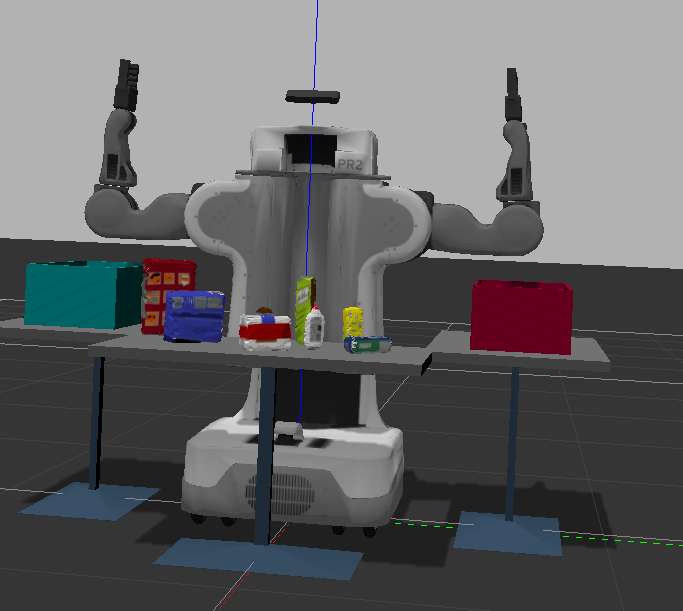
\includegraphics[totalheight=9cm]{imgs/title1.png}
\end{figure}}
\maketitle
In this project, we use point cloud data (from topic $/pr2/world/points$) and a perception pipeline to detect and identify objects on a table. The implementation of the pipeline involves multiple steps that are outlined in the sections below. The pipeline is used to identify a set of 3, 5 and 8 objects.

\section{Perception pipeline}

\subsection{Downsampling}
The first step consists in using a Voxel Grid Filter. The voxel size (\textit{LEAF\_SIZE}) is set to 0.01 m. A higher number results in a loss of resolution.

\linespread{1.3}
\lstinputlisting[language=Python]{codes/voxel.py}

\subsection{Filter noise}
Next, we use a statistical outlier filter to \textit{clean up} the point cloud: $i.e$  remove the noise. For each data point, we compute the distance from that point to all the $k$ neighboring points. Assuming a Gaussian distribution, the mean $\mu$ and standard deviation $\sigma$ are computed. Any points that are outside the range $\mu \pm x \times \sigma$ are labeled as outliers and removed from the point cloud. $x$ is a scaling factor of the standard deviation..

\begin{figure}[H]
\centering
        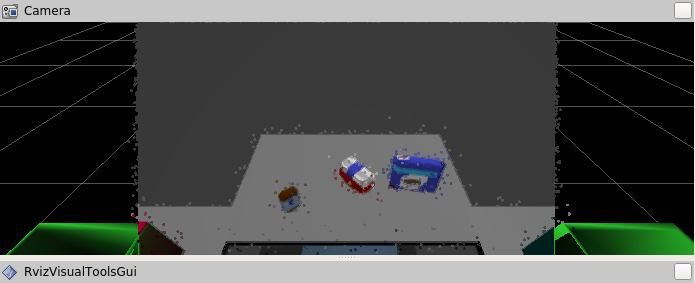
\includegraphics[totalheight=4cm]{imgs/p_original.png}
        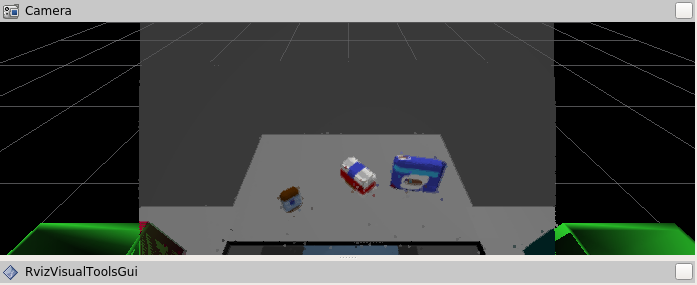
\includegraphics[totalheight=4cm]{imgs/p_remove_noise.png}
        \caption{Top image is the original point cloud, and bottom image is the point cloud after statistical outlier filtering.}
\end{figure}

In our implementation, we set the number of neighboring points to be $k=50$, and the scaling factor $x=0.1$.

\linespread{1.3}
\lstinputlisting[language=Python]{codes/noise_filter.py}

\subsection{Passthrough filter}
The passthrough filter is a \text{crop}-like method that enables to reduce the field of view. The first passthrough filter is along the $z$ axis, where only the points with $z$ coordinates in the range [0.6, 1.1] are preserved.
\newline

\linespread{0.5}
\lstinputlisting[language=Python]{codes/passthrough_z.py}

However, a single passthrough filter is not sufficient. In fact, the front edges of the 2 dropboxes remains in the view point of the camera and can alter the object recognition. Therefore, in addition of the $z$ axis passthrough, we also use a passthrough filter along the $y$ axis in the range [-0.35, 0.35].

\begin{figure}[H]
\centering
        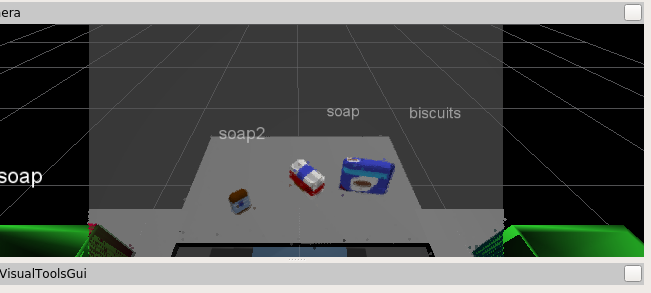
\includegraphics[totalheight=9cm]{imgs/p_z_passthrough.png}
        \caption{With a passthrough filter along z direction, there remains point clouds because related to the edges of the box (left and right). Those points can lead to erroneous recognition.}
\end{figure}

\linespread{1.3}
\lstinputlisting[language=Python]{codes/passthrough_z2.py}

\subsection{RANSAC}
In this step, we use RANSAC (Random Sample Consensus) algorithm to separate the objects and the table. The table is modeled as a plane to which we fit the entire  dataset. We can then extract 2 datasets: the inliers and the outliers. The inliers are the data points that follow the models and as a consequence are most likely associated with the table.

\begin{figure}[H]
\centering
        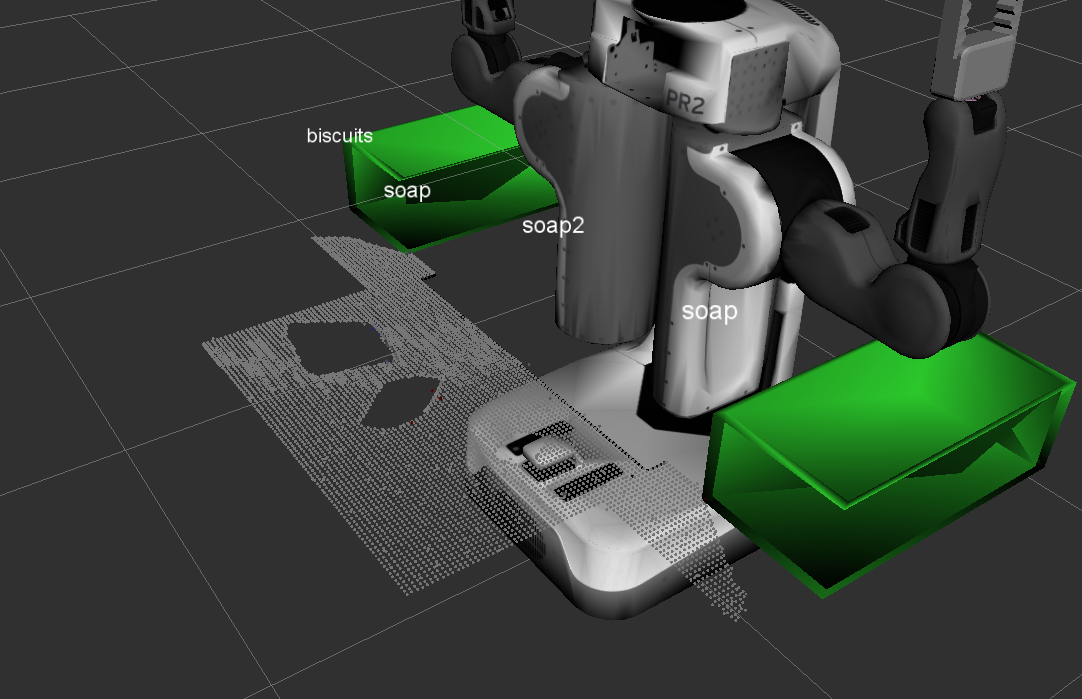
\includegraphics[totalheight=9cm]{imgs/ransac.png}
\end{figure}

\linespread{1.3}
\lstinputlisting[language=Python]{codes/ransac.py}

The hyper-parameter is the \textit{max\_distance}: it represents the maximum distance that the datapoint can be from the model best fit and still be considered to be an inlier. We set \textit{max\_distance}$=0.01$.

\subsection{Clustering (DBSCAN)}
The \textit{DBSCAN} (Density Based Spatial Clustering of Applications with Noise) is a unsupervised learning algorithm used for segmentation. The 2 hyper-parameters are \textit{min\_samples}, the minimum number of points that comprise a cluster, and \textit{max\_samples} is the maximum distance between cluster points.

\begin{figure}[H]
\centering
        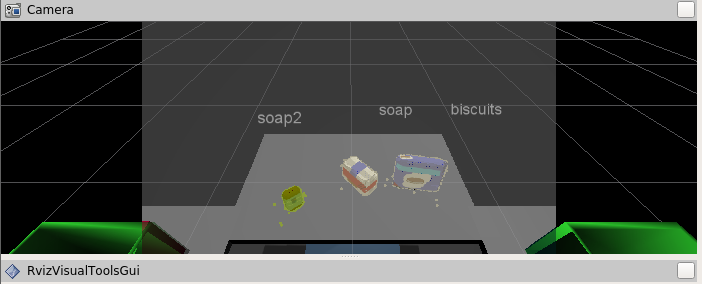
\includegraphics[totalheight=6cm]{imgs/cluster_1.png}
        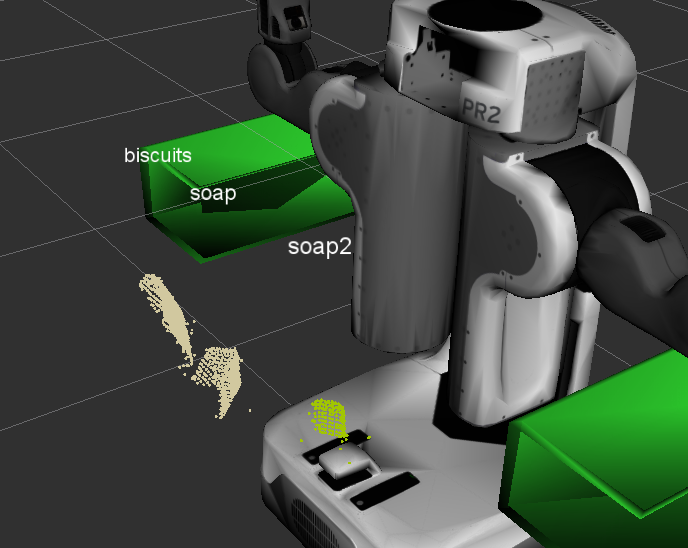
\includegraphics[totalheight=6cm]{imgs/cluster_2.png}
\end{figure}

\linespread{1.3}
\lstinputlisting[language=Python]{codes/clustering.py}

We set the tuning parameters as follows: \textit{cluster\_tolerance}$=0.05$, \textit{MinClusterSize}$=100$, \textit{MaxClusterSize}$=1550$.

\subsection{Object Recognition}
Now that we have segmented the point cloud, we need an algorithm to recognize the objects/segments. First, we need to define a set of features to characterize the objects, and then use a supervised learning algorithm to classify the clusters.

\subsubsection{Create features}
The features are composed of the color histogram and the normal surface histogram. The color histogram is constructed from the HSV channels, with the pixel intensity range [0, 255] splitted into 16 bins. The normal surface histogram has a range [0, 512] and 32 bins. The 2 histograms are then concatenated into a single vector and normalized.

\linespread{1.3}
\lstinputlisting[language=Python]{codes/features.py}


\subsubsection{Train model}
The classification algorithm is a Support Vector Machine. To train the model, we create a balanced dataset of different objects: $soap$, $soap2$ and $biscuits$ for example. We trained our model using features from 150 samples per category. The decision boundary can be either linear or non-linear, so the choice of the kernel in the \textit{SVM} affects the performance of the classifier. 
We ran a Grid search to find the best performing model:

\linespread{1.3}
\lstinputlisting[language=Python]{codes/gridsearch.py}

We also use a $K-fold$ cross validation to train the model. Such an approach is particularly useful when dealing with a small dataset. 

The best model is with \textit{kernel=linear}, $C=1$. 

\subsubsection{Results}
We trained 3 models depending on the number of objects t obe detected.
\begin{figure}[H]
\centering
        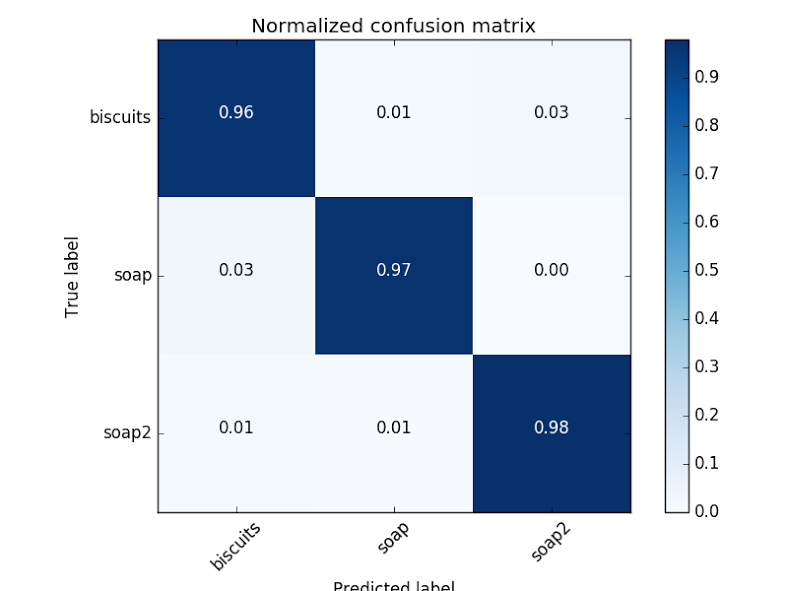
\includegraphics[totalheight=9cm]{imgs/test1.png}
        \caption{Normalized Confusion matrix for 3 objects (test1). The model has an accuracy of 96.89\%}
\end{figure}
     
\begin{figure}[H]
\centering
        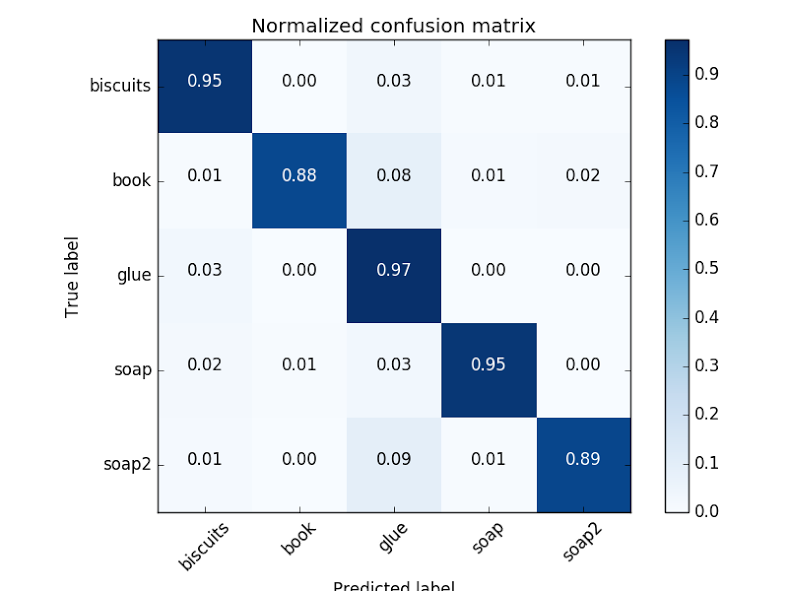
\includegraphics[totalheight=9cm]{imgs/test2.png}
         \caption{Normalized Confusion matrix for 5 objects (test2).  The model has an accuracy of 92.78\%}
\end{figure}

\begin{figure}[H]
\centering
        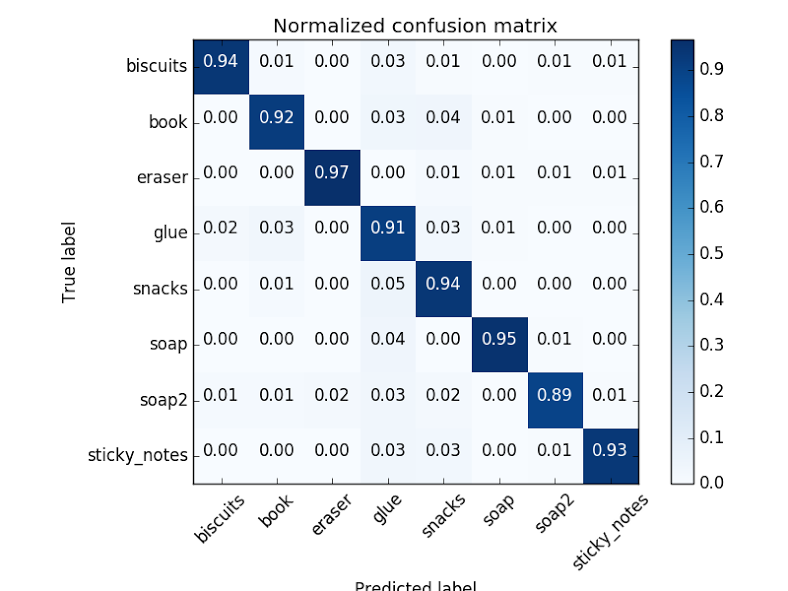
\includegraphics[totalheight=9cm]{imgs/test3.png}
        \caption{Normalized Confusion matrix for 8 objects (test3).  The model has an accuracy of 93\%}
\end{figure}

\section{Pipeline in action}
Below we show the output of the pipeline for the 3 worlds, where 3, 5 and 8 objects must be identified.

\begin{figure}[H]
\centering
        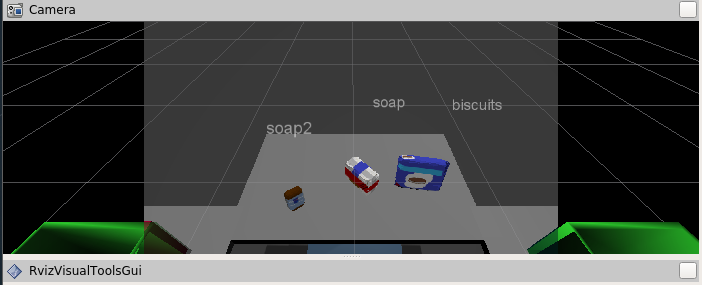
\includegraphics[totalheight=6cm]{imgs/result1.png}
        \caption{3 out of 3 objects correctly identified}
\end{figure}

\begin{figure}[H]
\centering
        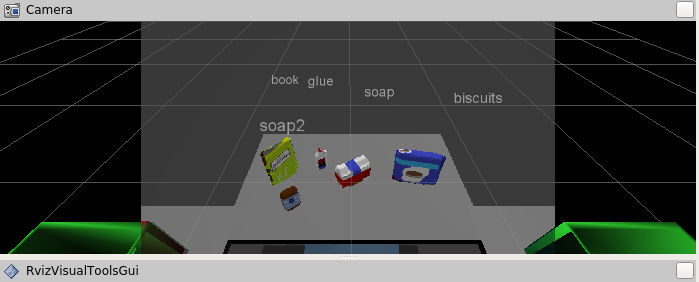
\includegraphics[totalheight=6cm]{imgs/result2.png}
        \caption{5 out of 5 objects correctly identified}
\end{figure}

\begin{figure}[H]
\centering
        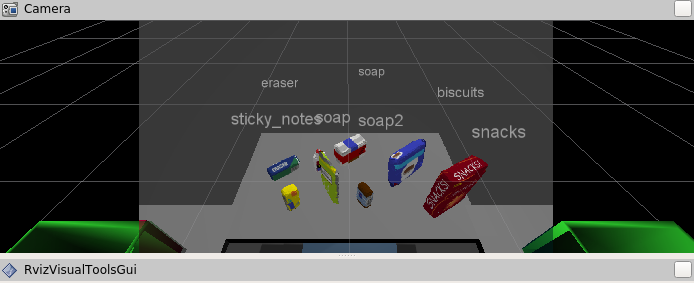
\includegraphics[totalheight=6cm]{imgs/result3.png}
        \caption{6 out of 8 objects correctly identified. The model cannot separate the glue and the book, and merged into a single cluster that it labels erroneously as soap.}
\end{figure}

\end{document}